\section{Introducción}

La Discalculia es una discapacidad de aprendizaje específica que afecta la adquisición de habilidades aritméticas. Aunque la falta de  enseñanza, recursos y la baja inteligencia se han relacionado con la etiología de la discalculia, se sabe actualmente que esta discapacidad del aprendizaje es un trastorno cerebral con una predisposición genética familiar \cite{Molko2003}.

\hfill

Por otra parte, hay estudios \cite{Molko2003,Shalev2001} que muestran que una forma de este fenotipo está asociado genéticamente con anomalías tanto funcionales como estructurales del surco intraparietal derecho, llevando esta región un papel fundamental en el desarrollo de las habilidades aritméticas.

\subsection{Búsqueda del fenotipo}

Para la obtención de más información, hemos utilizado HPO (Human Phenotype Ontology). Este es un vocabulario estandarizado de anomalías fenotípicas en enfermedades humanas que utiliza un fenotipado detallado/preciso para poder ser usado a nivel computacional.

\hfill

Tras realizar una búsqueda del fenotipo a investigar, \textit{Dyscalculia}, vemos que se encuentra clasificado como \href{https://hpo.jax.org/app/browse/term/HP:0002442}{HP:0002442} con un total de 13 fenotipos de otras enfermedades asociadas y un total de 24 genes asociados a esta en HPO.

\hfill

Gracias a las anotaciones en HPO, podemos obtener los genes asociados del fenotipo, y con ello podemos obtener información adicional: Ahoro procedemos a la búsqueda de más información a cerca de estos utilizando \href{https://string-db.org}{STRING}, una base de datos biológica y un recurso web de interacciones entre proteínas.

\begin{figure}[]
	\centering
	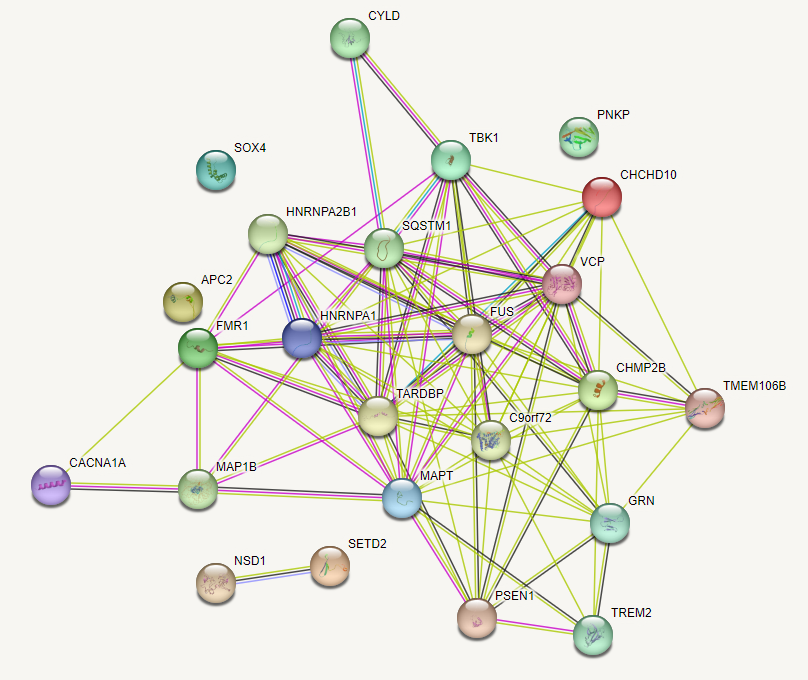
\includegraphics[width=0.50\textwidth]{figures/Gene-Relationships.PNG}
	\caption{Interacciones proteína-proteína a raíz de los genes relacionados. }
	\label{fig:string1}
\end{figure}


\hfill

\subsection{Búsqueda de interacciones}

Tras investigar las distintas interacciones proteína-proteína (véase la figura \ref{fig:string1}) y observar las enfermedades relacionadas con la discalculia en HPO y los distintos articulos científicos citados anteriormente, la estrecha relación de la discapacidad con un mal funcionamiento del sistema nervioso. En concreto se podría teorizar que existe una relación con las enfermedades de demencia del complejo frontotemporal del cerebro y la esclerosis lateral amiotrófica, pues estas palabras claves aparecen en la mitad de las enfermedades relacionadas con el fenotipo.

\hfill

Enfermedades como Alzheimer u otras que tienen que ver demencias fronto-temporales \cite{Walterfang2014} están también fuertemente relacionadas con un número significativo de proteínas relacionadas en la red de interacciones mencionada anteriormente.

\hfill

A raíz de los artículos recomendados por la base de datos STRING \cite{Walterfang2014,frontotemporal}, suponemos una relación de estos efectos negativos con una mala conexión entre los hemisferios cerebrales, recordemos que el cerebro delega algunas funciones clave como en este caso puede ser la realización de operaciones matemáticas o el reconocimiento numérico y las interconecta a través del Cuerpo Calloso \cite{CorpusCallosum}. Por tanto, un mal funcionamiento de este elemento del sistema puede llevar a una incapacidad de conexión de las funciones de los distintos hemisferios.

\hfill